\section{Modello di sviluppo} \label{section:modello_di_sviluppo}
Il gruppo ha deciso di lavorare secondo il \textbf{modello incrementale} per il \textit{ciclo di vita}\glo{} del software per i seguenti motivi:
\begin{itemize}
  \item Può produrre valore ad ogni incremento, aiutando a fissare meglio i requisiti per gli incrementi successivi;
  \item Ogni incremento riduce il rischio di fallimento;
  \item Le funzionalità principali sono sviluppate nei primi incrementi, rendendole via via più stabili.
\end{itemize}
Nel modello incrementale i requisiti vengono classificati in base alla loro importanza strategica. In questo modo, quelli più importanti vengono 
trattati prima. Questo ne aumenta la chiarezza e la facilità di soddisfazione. I requisiti meno importanti invece vengono soddisfatti in seguito, 
venendo così inseriti in un sistema già stabilizzato.\\
Il metodo di lavoro sarà quindi il seguente:
\begin{itemize}
  \item In ogni fase di lavoro vengono prefissati degli incrementi che devono essere prodotti entro una scadenza decisa dal gruppo;
  \item Il lavoro viene diviso tra i membri del gruppo;
  \item Al termine del periodo prefissato, servirà una riunione per analizzare il lavoro svolto da ogni membro, riscontrare problemi e difficoltà;
  \item Sarà compito dei \textit{verificatori} controllare il lavoro svolto dagli altri membri del gruppo e sollevare eventuali incongruenze o errori;
  \item Alla fine di questa verifica, seguirà una nuova discussione di gruppo per stabilire se gli obiettivi dell'incremento sono stati soddisfatti.
\end{itemize}

\begin{figure}[H]
	\centering
  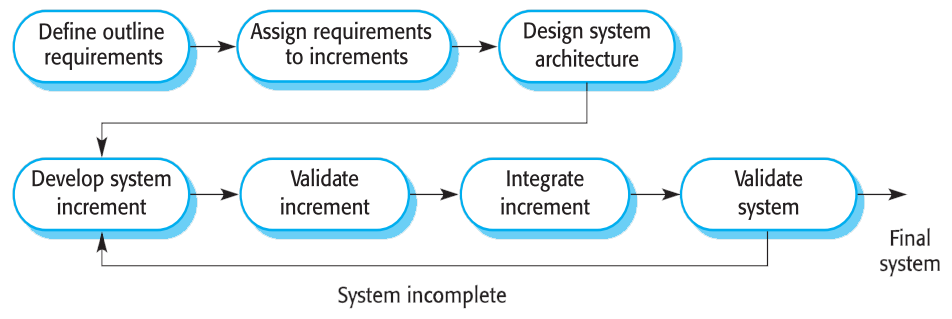
\includegraphics[scale=0.6]{immagini/modello_incrementale.png}
  \caption{Modello incrementale - tratto da: Ian Sommerville, \textit{Software Engineering}, 8th ed.}
\end{figure}
\pagebreak

%%%%%%%%%%%%%%%%%%%%%%%%%%%%%%%%%%%%%%%%%%%%%%%%%%%%%%%%%%%%%%%%%%%%%%%%%%%

\subsection{Incrementi individuati} \label{subsection:incrementi}
In seguito è riportata la tabella con indicati gli incrementi individuati, con il rispettivo obiettivo e i requisiti e casi d'uso ad esso associati. 
I requisiti riportati includono tutti i requisiti figli. Tutti i requisiti non riportati sono da intendersi soddisfatti, in parte, da 
ogni incremento. \\
Ogni requisito e caso d'uso è definito tramite il suo codice identificativo, per maggiori informazioni fare riferimento all'\docNameVersionAdR{}.

\begin{table}[H]
  \centering
  \renewcommand{\arraystretch}{1.8}
  \rowcolors{2}{green!100!black!40}{green!100!black!30}
  \begin{tabular}{c|p{6cm}|p{2cm}|p{2cm}}
    \rowcolor[HTML]{125E28}
    \color[HTML]{FFFFFF}\textbf{Incr.}
    & \multicolumn{1}{c}{\color[HTML]{FFFFFF}\textbf{Obiettivo}}
    & \multicolumn{1}{c}{\color[HTML]{FFFFFF}\textbf{Requisiti}}
    & \multicolumn{1}{c}{\color[HTML]{FFFFFF}\textbf{Casi d'uso}}\\
    \hline
    I	& Studio di Fantom\glo{} come blockchain\glo{} di riferimento e relative differenze con Ethereum\glo.	& R1V1\ \ \ \  R1V2 R2V4 R1V6 & \ \ \ \ \ \ \ - \\
    II & Studio librerie e pattern per lo sviluppo Frontend\glo{} di React. & R1V3\ \ \ \  R3V5 R1V7 & \ \ \ \ \ \ \ - \\
    III	& Stesura smart contract\glo{} per pagamento singolo e relativo modulo frontend\glo{} per l'interazione tramite Metamask. & R1F1\ \ \  R1F2 R1F2.1 R1F3\ \ \ \ R1F4\ \ \ \  R1F5 R1F5.1\ \ \ \  R1F7\ \ \ \  R1F8 & UC1\ \ \ \ \ \ \ UC2\ \ \ \ UC2.1\ \ \ \   UC3\ \ \ \ \ \ \ UC4\ \ \ \ \ \ UC4.1 UC4.2 UC4.3 UC4.4\ \ \ \ \ \ UC5\ \ \ \ UC5.1 UC5.2\ \ \ \ UC6\ \ \ \ \ \ \  UC7 \\
    IV & Studio e realizzazione del design con esaltazione dei diversi cambiamenti di stato. & \ \ \ \ \ \ \ - & \ \ \ \ \ \ \ - \\
    V	& Aggiunta di funzionalità Rimborso nello smart contract\glo{} e relativo modulo frontend\glo{} per l'interazione tramite Metamask\glo{}. & R1F6 & UC8 \\
    VI & Aggiunta di funzionalità MoneyBox\glo{} nello smart contract\glo{} e relativo modulo frontend\glo{} per l'interazione tramite Metamask\glo{}.  & R1F2.2 R2F2.2.1 R2F2.2.2 R2F2.2.4 R2F2.2.5 R2F5.2 & UC2.2 UC2.2.1 UC2.2.2 UC2.2.3 UC2.2.4 \\
  \end{tabular}
\end{table}
\begin{center}
  \textit{\small Continua nella pagina successiva}
\end{center}
\begin{table}[H]
  \centering
  \renewcommand{\arraystretch}{1.8}
  \rowcolors{2}{green!100!black!40}{green!100!black!30}
  \begin{tabular}{c|p{6cm}|p{2cm}|p{2cm}}
    \rowcolor[HTML]{125E28}
    \color[HTML]{FFFFFF}\textbf{Incr.}
    & \multicolumn{1}{c}{\color[HTML]{FFFFFF}\textbf{Obiettivo}}
    & \multicolumn{1}{c}{\color[HTML]{FFFFFF}\textbf{Requisiti}}
    & \multicolumn{1}{c}{\color[HTML]{FFFFFF}\textbf{Casi d'uso}}\\
    \hline
    VII	& Aggiunta di Ricerca, Paginazione e Filtrazione dell'elenco delle transazioni per maggiore fruibilità. & R2F8.1 R2F8.1.1 R2F8.1.2 R2F8.1.3 R1F8.2 R2F8.2.1 R2F8.2.2 R2F8.2.3 R2F8.2.4 & UC7.1 UC7.1.1 UC7.1.2 UC7.1.3 UC7.2 UC7.2.1 UC7.2.2 UC7.2.3 UC7.2.4 \\
    VIII & Aggiunta funzione dello smart contract\glo{} per la conversione del denaro in stable coin\glo{}. & R2F9 & \ \ \ \ \ \ \ - \\
    IX & Integrazione funzionalità d'identificazione grafica per i dati presenti in blockchain\glo{} e sviluppo punti opzionali restanti. & R3F2.2.3 R3F10  & \ \ \ \ \ \ \ - \\
  \end{tabular}
  \caption{Incrementi individuati}
\end{table}